\documentclass{article}

\usepackage[utf8]{inputenc}
\usepackage[english]{babel}
\usepackage{amsthm} %lets us use \begin{proof}
\usepackage{amssymb} %gives us the character \varnothing
\usepackage{xcolor}
\usepackage{float}
\usepackage{braket}
\usepackage{multirow}
\usepackage{array}
\usepackage{mathtools}
\usepackage{geometry}
\usepackage{graphicx}
\geometry{margin=1in}

\title{Chapter 2: Quantum Dynamics in Hilbert Space} % Title of the assignment

\begin{document}

\maketitle

\section{Overview}

Chapter 2 introduces the reader to the Time-Dependent Schr{\"o}dinger equation (TDSE)
and defines the time propagator operator ($U(t,t_0)$). The two level system is
provided as an example of solving the TDSE and the corresponding time propagator operator
is determined. The interaction picture is used to simplify the
problem from the Schr{\"o}dinger picture and various properties are shown. Lastly,
the Greens function within the frequency domain is used to model the proposed
Wigner and Weisskopy of irreversible decay.

\section{Time-Evolution Operator with Time-Dependent Hamiltonian}{\label{sec:setup}}

Within the Schr{\"o}dinger picture, the TD wavefunction in the position space $\mathbf{x}$
is given by
\begin{equation}
  \psi(\mathbf{x},t) = \langle \mathbf{x}|\psi(t)\rangle
\end{equation}
and the TDSE will be defined as
\begin{equation}
  \frac{\partial|\psi(t)\rangle}{\partial t} = -\frac{i}{\hbar}H|\psi(t)\rangle
  \label{eqn:tdse}
\end{equation}
and solutions to Eqn \eqref{eqn:tdse} are the eigenvectors $|\phi_n(t)\rangle$ with corresponding
eigenvalues $E_n$. These eigenvections form a complete basis set and satisfy the completness
condition $\sum_n|\phi_n\rangle\langle\phi_n|=1$. We can expand the wavefunction
$\psi(t)$ within this basis,
\begin{equation}
  |\psi(t)\rangle = \sum_n|\phi_n\rangle\langle\phi_n|\psi(t)\rangle.
  \label{eqn:basis_expand}
\end{equation}

Substitution of Eqn \eqref{eqn:basis_expand} into the TDSE yields
\begin{equation}
  \frac{d}{dt}\langle \phi_n|\psi(t)\rangle = -\frac{i}{\hbar}E_n\langle\phi_n|\psi(t)\rangle,
  \label{eqn:tdse_basis}
\end{equation}
which is 1st-order differential equation with the solution
\begin{equation}
  \langle\phi_n|\psi(t)\rangle = \sum_ne^{-\frac{iE_n}{\hbar}(t-t_0)}|\phi_n\rangle
  \langle\phi_n|\psi(t_0)\rangle.
  \label{eqn:time_soln}
\end{equation}

The general time evolution operator is defined as
\begin{equation}
  |\psi(t)\rangle = U(t,t_0)|\psi(t_0)\rangle.
  \label{eqn:time_op}
\end{equation}

A few properties of the time evolution operator are that $U(t_0,t_0)=1$
and unitary $U^{\dagger}U=1$. The usefulness of this operator provides the means to solve the
time evolution of the system in general without needing specific initial conditions.
Hence, the TDSE only needs to be solved once with the corresponding $U(t,t_0)$ which
may operate on any intial state $|\psi(t_0)\rangle$. Based on Eqn \eqref{eqn:time_soln} and
\eqref{eqn:time_op}, the time evolution operator is
\begin{equation}
  U(t,t_0) = \sum_n|\phi_n\rangle e^{-\frac{iE_n}{\hbar}(t-t_0)}\langle\phi_n|.
  \label{eqn:time_evol}
\end{equation}

The current form of $U(t,t_0)$ is limited to the representation of the Hamiltnian $H$
and a general form is provided for greater flexibility. This will allow semiclassical
approximations. The general form can be obtained by the concept of a function of an
operator via Taylor series expansion. Given function $f(A)$ for operator $A$, the Taylor
series can be seen as
\begin{align}
  f(A) \equiv \sum^{\infty}_{p=0}\frac{f^{(p)}(0)}{p!}x^p \\
  f(A) = \sum^{\infty}_{p=0}\frac{f^{(p)}(0)}{p!}x^p \equiv f(a_j)|\alpha_j\rangle\langle\alpha_j
  \label{eqn:op_func}
\end{align}

With Eqns \eqref{eqn:time_evol} and \eqref{eqn:op_func}, the $U(t,t_0)$ is recasted into the form
\begin{equation}
  U(t,t_0) = e^{-\frac{i}{\hbar}H(t-t_0)}.
\end{equation}

\subsection{Two-level System Example}

Section \ref{sec:setup} reviews the TD quantum mechanic equations and introduces the
generalized time evolution operator. With the tools, an example of the time evolution
operator is demonstrated for a coupled two-level system ($|\phi_a\rangle$ and $|\phi_b\rangle$),
with energies $\epsilon_a$ and $\epsilon_b$, and a coupling $V_{ab}$, represented by the
Hamiltonian
\begin{equation}
  H =
  \begin{pmatrix}
    \epsilon_a & V_{ab} \\
    V_{ba} & \epsilon_b
  \end{pmatrix}
  \label{eqn:two_level_H}
\end{equation}
where $V_{ab} - V*_{ba} = |V_{ab}|E^{-i\chi},\; 0 <\chi < 2\pi$. This can be made into
an eigenvalue problem
\begin{equation}
  H\begin{pmatrix}
  |\phi_a\rangle \\
  |\phi_b\rangle
  \end{pmatrix}
  =
  \begin{pmatrix}
    \epsilon_a & V_{ab} \\
    V_{ba} & \epsilon_b
  \end{pmatrix}
  \begin{pmatrix}
  |\phi_a\rangle \\
  |\phi_b\rangle
  \end{pmatrix}
  =\epsilon_{\pm}
  \begin{pmatrix}
  |\phi_a\rangle \\
  |\phi_b\rangle
  \end{pmatrix}
\end{equation}

Diagonalize the Hamiltonian,
\begin{align}
  \text{det}(H-\lambda\mathbf{1}) &= 0 \\
  (\epsilon_a-\lambda)(\epsilon_b-\lambda) - |V_{ab}|^2 &= 0 \\
  \lambda^2 -\lambda(\epsilon_a+\epsilon_b) + \epsilon_a\epsilon_b
  - |V_{ab}|^2 &= 0 \\
  \lambda &= \frac{(\epsilon_a+\epsilon_b) \pm
    \sqrt{(\epsilon_a+\epsilon_b)^2 -4\epsilon_a\epsilon_b + 4|V_{ab}|^2}}{2}\\
  & = \frac{(\epsilon_a+\epsilon_b) \pm
    \sqrt{(\epsilon_a-\epsilon_b)^2 + 4|V_{ab}|^2}}{2} \nonumber \\
\end{align}
Eigenvectors corresponding to eigenvalues $\lambda$ are
\begin{equation}
  \begin{pmatrix}
    \frac{\epsilon_a-\epsilon_b\pm\sqrt{(\epsilon_a-\epsilon_b)^2+4|V_{ab}|^2}}{2V} & 1
  \end{pmatrix}
  \label{eqn:theta}
\end{equation}
The corresponding generalized eigenvectors ($|\psi_{\pm}\rangle$) are simply
linear compinations of $|\phi_a\rangle$ and $|\phi_b\rangle$
with the associated radiation phase $e^{\pm i\chi}$. These are rotated eigenvectors
from Eqn \eqref{eqn:theta}
\begin{equation}
  \begin{pmatrix}
    |\psi_+\rangle \\
    |\psi_-\rangle
  \end{pmatrix}
  =
  \begin{pmatrix}
    \cos(\theta) & \sin(\theta) \\
    -\sin(\theta)& \cos(\theta)
  \end{pmatrix}
  \begin{pmatrix}
    e^{-i\chi/2}|\phi_a\rangle \\
    e^{i\chi/2}|\phi_b\rangle
  \end{pmatrix}
  =\begin{pmatrix}
  \cos(\theta)e^{-i\chi}|\phi_a\rangle + \sin(\theta) e^{i\chi}|\phi_b\rangle \\
  \cos(\theta)e^{-i\chi}|\phi_a\rangle - \sin(\theta) e^{i\chi}|\phi_b\rangle
  \end{pmatrix}
  \label{eqn:sup_eig}
\end{equation}

$\theta$ is a transformation angle that can be determined with Eqns
\eqref{eqn:theta} and \eqref{eqn:sup_eig}. The work is shown in the mathematica
notebook
\begin{equation}
  \tan 2\theta \equiv \frac{2|V_{ab}|}{\epsilon_a-\epsilon_b},\; 0<\theta<\pi/2
  \label{eqn:angle_transform}
\end{equation}

Within this basis, the time evolution operator is given by
\begin{equation}
  U(t,t_0) = |\psi_+\rangle e^{-\frac{i\lambda_+}{\hbar}(t-t_0)}\langle\psi_+|
  + |\psi_-\rangle e^{-\frac{i\lambda_-}{\hbar}(t-t_0)}\langle\psi_-|
  \label{eqn:time_2_level}
\end{equation}

\subsection{Progating the two-level system}

Suppose the system is at initial time $t_0=0$ in the $|\phi_a\rangle$ state
and the probability that the system is in $|\phi_b\rangle$ at time $t$.
\begin{equation}
  P_{ab}(t)\equiv |\langle\phi_b|\psi(t)\rangle|^2 = |\langle\phi_b|U(t,t_0)|\phi_a\rangle|^2
  \label{eqn:prob_time}
\end{equation}

The states $|\phi_a\rangle$ and $|\phi_b\rangle$ are defined as unit
vectors and the substitution of Eqn \eqref{eqn:time_2_level} into Eqn \eqref{eqn:prob_time}
will yield the probability to be in state $|\phi_b\rangle$ at a given time $t$.
From mathematica, the $P_{ab}(t)$ is given as
\begin{align}
  P_{ab}(t)&= \sin^2(2\theta)\sin^2\Bigg(\frac{\lambda_- - \lambda_+}{2\hbar}t\Bigg)
  \label{eqn:trig_identity}\\
  &=\frac{4|V_{ab}|^2}{4|V_{ab}|^2+(\epsilon_a-\epsilon_b)^2}
  \sin^2\Bigg(\sqrt{4|V_{ab}|+(\epsilon_a-\epsilon_b)^2}\frac{t}{2\hbar}\Bigg)
  \label{eqn:prob_final}
\end{align}

The step from Eqn \eqref{eqn:trig_identity} to \eqref{eqn:prob_final}
is using Eqn \eqref{eqn:angle_transform}, the trignometry identity
$\sin^22\theta + \cos^22\theta = 1$, and substituting in the eigenvalues $\lambda$.
This is left for the reader to derive. Figure \ref{fig:prob} is the plot of
the probability for various coupling constants $V_{ab}$.
\begin{align*}
  \Bigg(\tan 2\theta & =  \frac{2|V_{ab}|}{\epsilon_a-\epsilon_b}\Bigg)^2 \\
  \tan^2(2\theta) & = \frac{4|V_{ab}|^2}{(\epsilon_a-\epsilon_b)^2} \\
  \sin^2(2\theta) + \cos^2(2\theta) & = 1 \\
  \tan^2(2\theta) & = \frac{1}{\cos^2(2\theta)} - 1 \\
  & = \frac{4|V_{ab}|^2}{(\epsilon_a-\epsilon_b)^2} \\
  \frac{1}{\cos^2(2\theta)} & = \frac{4|V_{ab}|^2 + (\epsilon_a-\epsilon_b)^2}{(\epsilon_a-\epsilon_b)^2} \\
  \cos^2(2\theta) & = \frac{(\epsilon_a-\epsilon_b)^2}{4|V_{ab}|^2 + (\epsilon_a-\epsilon_b)^2} \\
  & = 1 - \sin^2(2\theta) \\
  \sin^2(2\theta) & = \frac{4|V_{ab}|}{4|V_{ab}|^2 + (\epsilon_a-\epsilon_b)^2}
\end{align*}
\begin{figure}[hbpt]
  \centering
  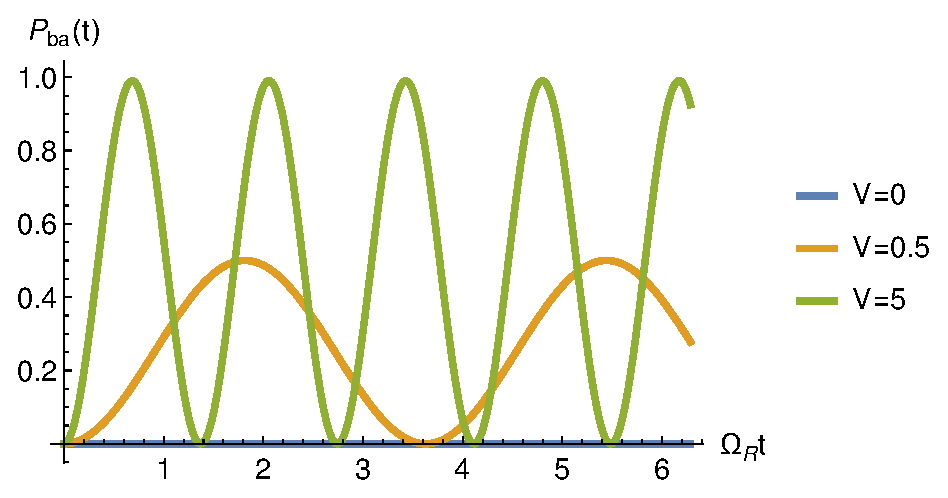
\includegraphics[scale=0.8]{prob2.eps}
  \caption{Rabi oscillation of the two level system for coupling constant $V_{ab}$ at 0, 0.5, and
  5.}
  \label{fig:prob}
\end{figure}
This is known as the Rabi formula and
\begin{equation}
  \Omega_{\text{R}}=\sqrt{4|V_{ab}|+(\epsilon_a-\epsilon_b)^2}/\hbar
\end{equation}
is the Rabi frequency.

\subsection{Propagation with Time-Dependent Hamiltonians: Time Ordering}

The generalize definition of the time-evolution operator to the time-dependent
Hamiltonian,
\begin{equation}
  \frac{\partial}{\partial t} U(t,t_0)|\psi(t_0)\rangle
  = - \frac{i}{\hbar}H(t)U(t,t_0)|\psi(t_0)\rangle.
  \label{eqn:time_int}
\end{equation}
Upon integration, the time propagator operator is
\begin{equation}
  U(t,t_0) = 1 - \frac{i}{\hbar}\int^t_{t_0}\,d\tau\,H(t)U(t,t_0).
  \label{eqn:int}
\end{equation}
Eqn \eqref{eqn:int} can be solved iteratively by plugging it into itself.
Iterating once, it becomes
\begin{equation}
  U(t,t_0) = 1 + \sum^{\infty}_{n=1}\Bigg(-\frac{i}{\hbar}\Bigg)^n
  \int^t_{t_0}d\tau_n\int^{\tau_n}_{t_0}d\tau_{n-1}\cdots\int^{\tau_2}_{t_0}
  d\tau_1H(\tau_n)H(\tau_{n-1})\cdots H(\tau_1)
  \label{eqn:time_order}
\end{equation}
Eqn \eqref{eqn:time_order} has the time variables as \textit{fully order}
$t\leq\tau_n\leq\cdots\leq\tau_1\leq_0$ and common to use a positive time
order exponential denoted as
\begin{equation}
  U(t,t_0) = e_+^{-\frac{i}{\hbar}\int^t_{t_0}d\tau H(\tau)}.
  \label{eqn:pos_time}
\end{equation}
Some cases may require taking the Hermitian conjugate
\begin{align}
  U^{\dagger}(t,t_0) = e_-^{\frac{i}{\hbar}\int^t_{t_0}d\tau H(\tau)}
  \label{eqn:conjugate_time}\\
  \langle\psi(t)| = \langle\psi(t)|U^{\dagger}(t,t_0)
\end{align}
Deriving eqn \eqref{eqn:conjugate_time} uses the hermiticity of the Hamiltonian
$H^{\dagger}(\tau)=H(\tau)$.

\section{Interaction Picture}

The time evolution operator is formally expressed and derived as follow
\begin{align}
  |\psi(t)\rangle & = U(t,t')U(t',t'')|\psi(t'')\rangle \\
  U(t,t'') & = U(t,t')U(t',t'')
\end{align}
The time operator can break it up as many times,
\begin{equation}
  U(t,t_0) = U(t,t_n)U(t_n,t_{n-1})\cdots U(t_1,t_0)
  \label{eqn:segs}
\end{equation}
This can be written into a large number $N$ of equal time segments $\delta t$
with $N\Delta t = t - t_0$. If $\Delta t$ is very small, then
\begin{equation}
  U(t_n,t_{n-1})\approx 1 - \frac{i}{\hbar}H(t_n)\Delta t.
  \label{eqn:inf_op}
\end{equation}
Introduced Eqn \eqref{eqn:inf_op} is the \textit{infinitesimal evolution operator}. Several properties
can be shown such as unitary operator and the total time evolution operator is
the product of infinitesimal evolution operator
\begin{align}
  U_{\text{tot}}(t,t_0) & = \Bigg[1-\frac{i}{\hbar}H(t_{n-1})\Delta t\Bigg]\Bigg[1-\frac{i}{\hbar}H(t_{n-2})\Delta t\Bigg]
  \cdots \Bigg[1-\frac{i}{\hbar}H(t_0)\Delta t\Bigg] \\
  & \approx 1 - \frac{i}{\hbar}\sum^n_{j=0}H(t_j)\Delta t + \cdots \\
  & \approx 1 - \frac{i}{\hbar}\int^t_{t_0}d\tau H(\tau)
\end{align}

The interaction picture allows the Hamiltonian to contain the zeroth order $H_0$
treated exactly while the remainder $H'(t)$ is expanded perturbatively. Let's
solve the $H_0$ exactly,
\begin{align}
  H(t) & = H_0(t) + H'(t) \\
  \frac{\partial}{\partial t}U_0(t,t_0) & = -\frac{i}{\hbar}H_0(t)U_0(t,t_0) \\
  U_0(t,t_0) & = e_+^{-\frac{i}{\hbar}\int^t_{t_0}d\tau H_0(\tau)}
\end{align}
The solution of the $U_0(t,t_0)$ lead to the definition of the interaction
picture wavefunction $|\psi_{\text{I}}(t)\rangle$
\begin{equation}
  |\psi_S(t)\rangle\equiv U_0(t,t_0)|\psi_I(t)\rangle
  \label{eqn:int_wave}
\end{equation}
where $|\psi_S(t)\rangle$ is the Schr{\"o}dinger picture wavefunction.
Substituion of the interaction picture wavefunction into the TDSE yields
\begin{align}
  \frac{\partial |\psi_I(t)\rangle}{\partial t} & = -\frac{i}{\hbar}H'_I(t)|\psi_I(t)\rangle
  \label{eqn:int_s}\\
  H'_I(t) & \equiv U_0^{\dagger}(t,t_0)H'(t)U_0(t,t_0)
\end{align}
The time propagator operator is introduced within the interaction representation
\begin{equation}
  |\psi_I(t)\rangle \equiv U_I(t,t_0)|\psi(t_0)\rangle
  \label{eqn:time_prop_int}
\end{equation}
Upon substituting Eqn \eqref{eqn:time_prop_int} into Eqn \eqref{eqn:int_s} to
get
\begin{align}
  \frac{\partial}{\partial t} U_I(t,t_0) & = -\frac{i}{\hbar}H'_I(t)U_I(t,t_0) \\
  U_I(t,t_0) & = e_+^{-\frac{i}{\hbar}\int^t_{t_0}d\tau H'_I(\tau)}
  \label{eqn:int_time_soln}
\end{align}
Looking back at the Schr{\"o}dinger picture, the time propagator operator $U(t,t_0)$
can be derived
\begin{align}
  |\psi_S(t)\rangle & = U_0(t,t_0)|\psi_I(t)\rangle \\
  & = U_0(t,t_0)U_I(t,t_0)|\psi_I(t_0)\rangle \\
  & = U_0(t,t_0)U_I(t,t_0)|\psi_S(t_0)\rangle
\end{align}
At initial time $t_0$, the $|\psi_I(t_0)\rangle = |\psi_S(t_0)\rangle$ and hence,
the $U(t,t_0)$ becomes
\begin{align}
  U(t,t_0) & = U_0(t,t_0)U_I(t,t_0) \\
  & = U_0(t,t_0)e_+^{-\frac{i}{\hbar}\int_{t_0}^td\tau H'_I(t)}
\end{align}
As long as $H_0$ and $U_0(t,t_0)$ are expressed exactly, the time operator
may be expanded in powers of $H'(\tau)$ alone
\begin{equation}
  U(t,t_0) = U_0(t,t_0) + \sum^{\infty}_{n=1}\Bigg(-\frac{i}{\hbar}\Bigg)^n
  \int^t_{t_0}d\tau_n\cdots\int^{\tau_2}_{t_0}d\tau_1
  U_0(t,\tau_n)H'(\tau_n)U_0(\tau_n\tau_{n-1})\cdots U_0(\tau_2,\tau_1)H'(\tau_2)U_0(\tau_1,t_0).
  \label{eqn:full_time_int}
\end{equation}
All time ordering is satisfied by Eqn \eqref{eqn:full_time_int}. The result
may be interpreted as the system propogating freely from time $t_0$ to $\tau_1$
with $U_0(\tau_1,t_0)$ and then interacts with $H'(\tau_1)$ from time $\tau_1$
to $\tau_2$ with $U_0(\tau_2,\tau_1)$ and etc. In addition, this form allow
truncation at low order and propagation at long time. The corresponding wavefunction
can be determine up to first order
\begin{equation}
  |\psi(t)\rangle = |\psi_0(t)\rangle - \frac{i}{\hbar}\int^t_{t_0}
  d\tau U_0(t,\tau)H'(\tau)|\psi(\tau)\rangle
\end{equation}
where
\begin{equation}
  |\psi_0(t)\rangle\equiv U_0(t,t_0)|\psi_S(t_0)\rangle
\end{equation}

\subsection{Properties of Interaction Picture}

The interaction picture has a significant meaning for a given operator $A$
defined as
\begin{equation}
  A_I(t)\equiv U^{\dagger}_0(t,t_0)A_SU(t,t_0)
  \label{eqn:op_int}
\end{equation}
Time evolution in the interaction picture is given by
\begin{align}
  \langle A(t)\rangle & = \langle \psi_I(t)|A_I(t)|\psi_I(t)\rangle \\
  \frac{\partial \psi_I}{\partial t} & = -\frac{i}{\hbar}H'_I(t)\psi_I \\
  \frac{\partial A_I}{\partial t} & = \frac{i}{\hbar}[H_0,A_I] \\
  H'_I(t) & = U^{\dagger}_0(t,t_0)H'(t)U_0(t,t_0)
\end{align}
These equations are valid for an arbitrary partitioning of the Hamiltonian.
For instance, choosing the $H_0=0$ and $H'=H$ yield the \textit{Schr{\"o}dinger
  picture} where the time evolution is entirely with the wavefunction and the
operators are time independent. Moreover, a choice of $H_0=H$ and H'=0 yields
the \textit{Heisenberg picture} where the wavefunction is time independent and
the entire evolution is with the operator. Meanwhile, the interaction picture
is the mix beteween the \textit{Schr{\"o}dinger} and \textit{Heisenberg pictures}.

\subsection{Magnus Expansion}
The application of the cumulant expansion on the time evolution operator in the
interaction picture and expressed the time-ordered exponential of $H'_I$ as an
ordinary exponential of a different, time-dependent operator, given by an infinite
series.
\begin{equation}
  U_I(t,t_0) = e_+^{-i/\hbar\int_0^t\,d\tau H_I'(\tau)} \equiv
    e^{\sum_{n=1}^{\infty}(1/n!)(-i/\hbar)^nH_n(t,t_0)}
\end{equation}
where
\begin{align}
  H_1 & = \int_{t_0}^t d\tau_1 H_I'(\tau_1) \\
  H_2 & = \int_{t_0}^t d\tau_2 \int_{t_0}^{t_2} d\tau_1 [H_I'(\tau_2),H_I'(\tau_1)] \\
  H_3 & = \int_{t_0}^t d\tau_3 \int_{t_0}^{t_3} d\tau_2 \int_{t_0}^{t_2} d\tau_1
  \{[H_I'(\tau_3),[H_I'(\tau_2),H_I'(\tau_1)]] + [[H_I'(\tau_3),H_I'(\tau_2)],H_I'(\tau_1)]\}.
\end{align}

\section{Green Function and Casuality}
Casuality describes that in the natural science, the effect does not come before
the cause. An example is that the effect of a ball moving happens due to a force
causing it to move. With the time evolution operator $U(t,t_0)$, it is useful to
work in the frequency domain rather than the time domain. This unitary transformation
is done by the Green function which separates the forward ($t>t_0$) and reverse ($t<t_0$)
propagations.
\begin{align}
  G(t-t_0) & \equiv \theta(t-t_0)U(t,t_0) \\
  & = \theta(t-t_0)E^{(-i/\hbar)H(t-t_0)} \nonumber
\end{align}
where $\theta(t-t_0)$ is the Heavyside step function. Contour integration yields
\begin{align}
  \theta(t-t_0)U(t,t_0) 7 & = -\frac{1}{2\pi i}\int_{-\infty}^{\infty} dE e^{-(i/\hbar)E(t-t_0)}G(E) \\
  G(E) & = \sum_n \frac{|\phi_n\rangle\langle\phi_n|}{E-E_n+i\epsilon}
\end{align}

Once in this form, perturbative expansion can be conveniently carried out using
the Green functio which satisfy the Dyson equation. The zero order Green function
\begin{equation}
  G_0(E) = \frac{1}{E-H_0+i\epsilon}
\end{equation}
where $H = H_0 + V$. Using the identity $A^{-1} = B^{-1}(B-A)A^{-1}$, where
$A$ and $B$ are operators, then
\begin{align}
  G(E) & = G_0(E) + G_0(E)VG(E) \\
  G(E) & = G_0(E) + G_0(E)VG_0(E) + G_0(E)VG_0(E)VG_0(E) + \cdots
\end{align}
Keep in mind, $G_0(E)$ is a diagonal matrix while $V$ is an off-diagonal matrix.


\end{document}
